% PL-template.tex
% Copyright 2016 Guido Vanden Wyngaerd
% Copyright 2026 Philosophical Logic editorial team
%
% This file is a modified version of the Glossa LaTeX template from Glossalatex: https://github.com/guidovw/Glossalatex
%
% This derived work may be distributed and/or modified under the conditions of the LaTeX Project Public License, version 1.3 or later.
% The latest version of this license is at https://www.latex-project.org/lppl.txt, and version 1.3 or later is part of all distributions of LaTeX version 2005/12/01 or later.
%
% This derived work has the LPPL maintenance status `maintained'.
%
% The Current Maintainer of this derived work is the Philosophical Logic editorial team. Contact: editorial@philosophical-logic.org.
% The original Glossa work is maintained by Guido Vanden Wyngaerd; the original maintainer does not provide support for this derived work.
%
% This derived work consists of the files
% PL.cls
% PL.bst
% PL-template.tex
%
% Licensing and modification details: LICENSE.md.

% INITIAL SUBMISSION (the default): use the class with no option.
% The class hides the author block and clears PDF author metadata for double-anonymous review.
% After acceptance, use \documentclass[accepted]{PL} to display the author information supplied below.
\documentclass{PL}
\usepackage{tikz}
\usetikzlibrary{arrows.meta}

% See README.md and AUTHOR-GUIDE.md for compilation and submission guidance.

\newtheorem{theorem}{Theorem}[section]
\newtheorem{lemma}[theorem]{Lemma}
\theoremstyle{definition}
\newtheorem{definition}[theorem]{Definition}

% Supply real author data here. It remains in the source but is not printed or written to PDF metadata in the default anonymous mode.
\pdfauthor{Author One and Author Two}
\pdftitle{A Sample Philosophical Logic Article}
\pdfkeywords{modal logic, logical consequence, possible worlds}

% Use Title Case for an English article title. The optional short title is used in running heads.
\title[Sample Philosophical Logic Article]{A Sample Philosophical Logic Article}

\author[Author One \& Author Two]{%
  \spauthor{Author One\\
    \institute{Institution One}\\
    \small{\email{author.one@example.edu}}}
  \AND%
  \spauthor{Author Two\\
    \institute{Institution Two}\\
    \small{\email{author.two@example.edu}}}%
}

\begin{document}

\maketitle

\begin{abstract}
This concise sample illustrates the structure of a submission to \emph{Philosophical Logic}, including citations, formal material, floats, and back matter. Replace this text with a self-contained summary of the article's question, approach, principal result, and significance.
\end{abstract}

\begin{keywords}
modal logic; logical consequence; possible worlds
\end{keywords}

\section{Introduction}

The journal uses double-anonymous review. The default class mode therefore omits the author block even though author data are present in the source. Authors must still remove identifying prose and anonymize links or citations that would reveal their identity.

Number sections and subsections, and write English section headings in sentence case. Use ordinary cross-references rather than references to material ``above'' or ``below''; for example, equation~\eqref{eq:box}, Theorem~\ref{thm:k-valid}, Table~\ref{tab:correspondence}, and Figure~\ref{fig:frame} will remain identifiable if floats move during typesetting.

\section{A sample formal result}

Use standard \LaTeX\ commands for mathematical notation. For a Kripke model $\mathcal{M}=\langle W,R,V\rangle$, the modal clause is
\begin{equation}
  \mathcal{M},w \models \Box\varphi
  \quad\Longleftrightarrow\quad
  \forall v\in W\,(wRv\Rightarrow\mathcal{M},v\models\varphi).
  \label{eq:box}
\end{equation}

Introduce nonstandard notation before using it, and check every formula and derivation carefully. Very wide proofs or displays should be reorganized to fit the page.

\begin{theorem}\label{thm:k-valid}
The axiom schema $\Box(p\rightarrow q)\rightarrow(\Box p\rightarrow\Box q)$ is valid on every Kripke frame.
\end{theorem}

\begin{proof}
At any world, if every accessible world satisfies $p\rightarrow q$ and every accessible world satisfies $p$, then every accessible world satisfies $q$. The claim follows from equation~\eqref{eq:box}.
\end{proof}

\section{Citations and references}

The class loads \texttt{natbib} and selects the journal's \texttt{PL.bst} bibliography style. Do not load \texttt{natbib} yourself, and do not add a \verb|\bibliographystyle| command. Use \verb|\citet| for a textual citation, as in \citet{marcus:1961}, and \verb|\citep| for a parenthetical citation, as in \citep{haack:1976}.

Within a grouped citation, list the bibliography keys in chronological order: the following source code lists work from 1936 through 1977 \citep{tarski:1936,marcus:1961,kripke:1963,lewis:1973,haack:1976,fischer-servi:1977}. Protect capitals that must remain uppercase in a \texttt{.bib} title by enclosing them in braces, for example \verb|{S5}| or \verb|{Kripke}|.

\section{Tables and figures}

Include every table and figure needed for review in the submitted PDF, cite each one in the text, and give each a descriptive caption. Table~\ref{tab:correspondence} gives a compact example.

\begin{table}[tb]
  \centering
  \begin{tabular}{lll}
    \toprule
    Frame condition & Formula schema & Standard name \\
    \midrule
    Reflexive  & $\Box p\rightarrow p$                  & T \\
    Transitive & $\Box p\rightarrow\Box\Box p$         & 4 \\
    Symmetric  & $p\rightarrow\Box\Diamond p$          & B \\
    \bottomrule
  \end{tabular}
  \caption{Sample modal correspondence table}%
  \label{tab:correspondence}
\end{table}

The diagram in Figure~\ref{fig:frame} is drawn with TikZ, so the template does not depend on an external image file. Authors may instead use \verb|\includegraphics| and should retain editable or high-resolution source files for accepted manuscripts.

\begin{figure}[tb]
  \centering
  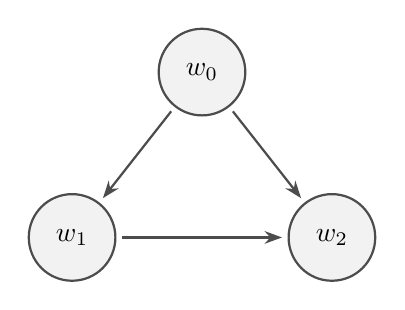
\begin{tikzpicture}[
    world/.style={
      circle,
      draw=black!70,
      fill=black!5,
      line width=0.8pt,
      minimum size=11mm,
      inner sep=0pt
    },
    access/.style={
      -{Stealth[length=2.2mm,width=1.6mm]},
      draw=black!70,
      line width=0.8pt,
      shorten <=2pt,
      shorten >=2pt
    }
  ]
    \node[world] (w0) at (0,1.35) {$w_0$};
    \node[world] (w1) at (-1.65,-0.75) {$w_1$};
    \node[world] (w2) at (1.65,-0.75) {$w_2$};

    \draw[access] (w0) -- (w1);
    \draw[access] (w0) -- (w2);
    \draw[access] (w1) -- (w2);
  \end{tikzpicture}
  \caption{A three-world Kripke frame}%
  \label{fig:frame}
\end{figure}

\section{Conclusion}

The conclusion is normally the last numbered section. Keep the back matter that follows concise, use only the optional headings relevant to the article, and consult the live journal and publisher policies before submission: \href{https://www.philosophical-logic.org/site/journal-policies/}{journal policies} and \href{https://www.philosophical-logic.org/site/author-guidelines/}{author guidelines}.

% OPTIONAL BACK MATTER
% Uncomment only the sections that apply. Omit or anonymize identifying material during anonymous review.

% \section*{Ethics and consent}
% [Statement, if applicable.]

% \section*{Data availability}
% [Statement, if applicable.]

% \section*{AI declaration statement}
% [Statement, if required by current OLH policy.]

% \section*{Funding information}
% [Statement, if applicable.]

% \section*{Acknowledgements}
% [Statement, if applicable.]

% \section*{Authors' contributions}
% [Statement, if applicable.]

% REQUIRED BACK MATTER
\section*{Competing interests}

The authors declare that they have no competing interests.

% Replace `sample' with the name of your own .bib file. PL.cls supplies the required \bibliographystyle{PL} command; do not add another one here.
\bibliography{sample}

\end{document}
